\documentclass[a4paper, 14pt]{extarticle}

\usepackage{tikz}
\usepackage{aeguill}

% Поля
%--------------------------------------
\usepackage{geometry}
\geometry{a4paper,tmargin=2cm,bmargin=2cm,lmargin=3cm,rmargin=1cm}
%--------------------------------------


%Russian-specific packages
%--------------------------------------
\usepackage[T2A]{fontenc}
\usepackage[utf8]{inputenc} 
\usepackage[english, main=russian]{babel}
%--------------------------------------

\usepackage{textcomp}
% § for list
\usepackage{easylist}

% Красная строка
%--------------------------------------
\usepackage{indentfirst}               
%--------------------------------------             


%Graphics
%--------------------------------------
\usepackage{graphicx}
\graphicspath{ {./images/} }
\usepackage{wrapfig}
%--------------------------------------

% Полуторный интервал
%--------------------------------------
\linespread{1.3}                    
%--------------------------------------

% Таблицы
\usepackage{longtable}

%Выравнивание и переносы
\usepackage{tabularx}
% ragged X column for wrapping long text in table cells
\newcolumntype{Y}{>{\raggedright\arraybackslash}X}
%--------------------------------------
% Избавляемся от переполнений
\sloppy
% Запрещаем разрыв страницы после первой строки абзаца
\clubpenalty=10000
% Запрещаем разрыв страницы после последней строки абзаца
\widowpenalty=10000
%--------------------------------------

%Списки
\usepackage{enumitem}

%Подписи
\usepackage{caption} 

%Гиперссылки
\usepackage{hyperref}

\hypersetup {
    unicode=true,
    colorlinks=true,
    linkcolor=black,
    filecolor=magenta,      
    urlcolor=cyan,
}

%Рисунки
%--------------------------------------
\DeclareCaptionLabelSeparator*{emdash}{~--- }
\captionsetup[figure]{labelsep=emdash,font=onehalfspacing,position=bottom}
%--------------------------------------

\usepackage{tempora}

%Листинги
%--------------------------------------
\usepackage{listings}

\lstset{
  basicstyle=\ttfamily\footnotesize, 
  %basicstyle=\footnotesize\AnkaCoder,        % the size of the fonts that are used for the code
  breakatwhitespace=false,         % sets if automatic breaks shoulbd only happen at whitespace
  breaklines=true,                 % sets automatic line breaking
  captionpos=t,                    % sets the caption-position to bottom
  inputencoding=utf8,
  frame=single,                    % adds a frame around the code
  keepspaces=true,                 % keeps spaces in text, useful for keeping indentation of code (possibly needs columns=flexible)
  keywordstyle=\bf,       % keyword style
  numbers=left,                    % where to put the line-numbers; possible values are (none, left, right)
  numbersep=5pt,                   % how far the line-numbers are from the code
  xleftmargin=25pt,
  xrightmargin=25pt,
  showspaces=false,                % show spaces everywhere adding particular underscores; it overrides 'showstringspaces'
  showstringspaces=false,          % underline spaces within strings only
  showtabs=false,                  % show tabs within strings adding particular underscores
  stepnumber=1,                    % the step between two line-numbers. If it's 1, each line will be numbered
  tabsize=2,                       % sets default tabsize to 8 spaces
  title=\lstname                   % show the filename of files included with \lstinputlisting; also try caption instead of title
  % Для отображения русского языка
  extendedchars=true,
  literate={Ö}{ {\"O} }1
  {Ä}{ {\"A} }1
  {Ü}{ {\"U} }1
  {ß}{ {\ss} }1
  {ü}{ {\"u} }1
  {ä}{ {\"a} }1
  {ö}{ {\"o} }1
  {~}{ {\textasciitilde} }1
  {а}{ {\selectfont\char224} }1
  {б}{ {\selectfont\char225} }1
  {в}{ {\selectfont\char226} }1
  {г}{ {\selectfont\char227} }1
  {д}{ {\selectfont\char228} }1
  {е}{ {\selectfont\char229} }1
  {ё}{ {\"e} }1
  {ж}{ {\selectfont\char230} }1
  {з}{ {\selectfont\char231} }1
  {и}{ {\selectfont\char232} }1
  {й}{ {\selectfont\char233} }1
  {к}{ {\selectfont\char234} }1
  {л}{ {\selectfont\char235} }1
  {м}{ {\selectfont\char236} }1
  {н}{ {\selectfont\char237} }1
  {о}{ {\selectfont\char238} }1
  {п}{ {\selectfont\char239} }1
  {р}{ {\selectfont\char240} }1
  {с}{ {\selectfont\char241} }1
  {т}{ {\selectfont\char242} }1
  {у}{ {\selectfont\char243} }1
  {ф}{ {\selectfont\char244} }1
  {х}{ {\selectfont\char245} }1
  {ц}{ {\selectfont\char246} }1
  {ч}{ {\selectfont\char247} }1
  {ш}{ {\selectfont\char248} }1
  {щ}{ {\selectfont\char249} }1
  {ъ}{ {\selectfont\char250} }1
  {ы}{ {\selectfont\char251} }1
  {ь}{ {\selectfont\char252} }1
  {э}{ {\selectfont\char253} }1
  {ю}{ {\selectfont\char254} }1
  {я}{ {\selectfont\char255} }1
  {А}{ {\selectfont\char192} }1
  {Б}{ {\selectfont\char193} }1
  {В}{ {\selectfont\char194} }1
  {Г}{ {\selectfont\char195} }1
  {Д}{ {\selectfont\char196} }1
  {Е}{ {\selectfont\char197} }1
  {Ё}{ {\"E} }1
  {Ж}{ {\selectfont\char198} }1
  {З}{ {\selectfont\char199} }1
  {И}{ {\selectfont\char200} }1
  {Й}{ {\selectfont\char201} }1
  {К}{ {\selectfont\char202} }1
  {Л}{ {\selectfont\char203} }1
  {М}{ {\selectfont\char204} }1
  {Н}{ {\selectfont\char205} }1
  {О}{ {\selectfont\char206} }1
  {П}{ {\selectfont\char207} }1
  {Р}{ {\selectfont\char208} }1
  {С}{ {\selectfont\char209} }1
  {Т}{ {\selectfont\char210} }1
  {У}{ {\selectfont\char211} }1
  {Ф}{ {\selectfont\char212} }1
  {Х}{ {\selectfont\char213} }1
  {Ц}{ {\selectfont\char214} }1
  {Ч}{ {\selectfont\char215} }1
  {Ш}{ {\selectfont\char216} }1
  {Щ}{ {\selectfont\char217} }1
  {Ъ}{ {\selectfont\char218} }1
  {Ы}{ {\selectfont\char219} }1
  {Ь}{ {\selectfont\char220} }1
  {Э}{ {\selectfont\char221} }1
  {Ю}{ {\selectfont\char222} }1
  {Я}{ {\selectfont\char223} }1
  {і}{ {\selectfont\char105} }1
  {ї}{ {\selectfont\char168} }1
  {є}{ {\selectfont\char185} }1
  {ґ}{ {\selectfont\char160} }1
  {І}{ {\selectfont\char73} }1
  {Ї}{ {\selectfont\char136} }1
  {Є}{ {\selectfont\char153} }1
  {Ґ}{ {\selectfont\char128} }1
  % \definecolor{brackets}{HTML}{B40000} % цвет скобок в коде
  % {\{}{ { {\color{brackets}\{} } }1 % Цвет скобок {
  % {\} }{ { {\color{brackets}\} } } }1 % Цвет скобок }
}

%--------------------------------------

% Table of contents
\usepackage{tocloft}
\usepackage{adjustbox}
\renewcommand{\cftpartleader}{\cftdotfill{\cftdotsep}} % for parts
\renewcommand{\cftsecleader}{\cftdotfill{\cftdotsep}} % for sections, if you really want! (It is default in report and book class (So you may not need it).

\usepackage{titlesec}
\titleformat{\paragraph} % Format the paragraph command
[hang] % Shape
{\normalfont\normalsize\bfseries} % Format for the text
{} % Label (we leave this empty to remove the number)
{0em} % Horizontal separation between label and title
{} % Code before the title body

% --- REDUCE PARAGRAPH INDENT IN TOC ---
% Reduce the space before the paragraph number (if numbered)
\setlength{\cftparaindent}{3em} % Default is often 2.5em or larger
% Reduce the box reserved for the paragraph number
% \setlength{\cftparanumwidth}{2.3em} % Default is often 3.0em
% \setlength{\cftparanumwidth}{0em}

% THIS IS THE CRUCIAL LINE: Set depth to 4 (paragraph) or even 5 (subparagraph)
\setcounter{tocdepth}{4} % 4 = paragraph, 5 = subparagraph
% --------------------------------------

%%% Математические пакеты %%%
%--------------------------------------
\usepackage{amsthm,amsfonts,amsmath,amssymb,amscd}  % Математические дополнения от AMS
\usepackage{mathtools}                              % Добавляет окружение multlined
\usepackage[perpage]{footmisc}
%--------------------------------------

%--------------------------------------
%			НАЧАЛО ДОКУМЕНТА
%--------------------------------------

\begin{document}

%--------------------------------------
%			ТИТУЛЬНЫЙ ЛИСТ
%--------------------------------------
\begin{titlepage}
\thispagestyle{empty}
\newpage


%Шапка титульного листа
%--------------------------------------
\vspace*{-60pt}
\hspace{-65pt}
\begin{minipage}{0.3\textwidth}
\hspace*{-20pt}\centering

\includegraphics[width=\textwidth]{emblem}
\end{minipage}
\begin{minipage}{0.67\textwidth}\small \textbf{
\vspace*{-0.7ex}
\hspace*{-6pt}\centerline{Министерство науки и высшего образования Российской Федерации}
\vspace*{-0.7ex}
\centerline{Федеральное государственное бюджетное образовательное учреждение }
\vspace*{-0.7ex}
\centerline{высшего образования}
\vspace*{-0.7ex}
\centerline{<<Московский государственный технический университет}
\vspace*{-0.7ex}
\centerline{имени Н.Э. Баумана}
\vspace*{-0.7ex}
\centerline{(национальный исследовательский университет)>>}
\vspace*{-0.7ex}
\centerline{(МГТУ им. Н.Э. Баумана)}}
\end{minipage}
%--------------------------------------

%Полосы
%--------------------------------------
\vspace{-25pt}
\hspace{-35pt}\rule{\textwidth}{2.3pt}

\vspace*{-20.3pt}
\hspace{-35pt}\rule{\textwidth}{0.4pt}
%--------------------------------------

\vspace{1.5ex}
\hspace{-35pt} \noindent \small ФАКУЛЬТЕТ\hspace{80pt} <<Информатика и системы управления>>

\vspace*{-16pt}
\hspace{47pt}\rule{0.83\textwidth}{0.4pt}

\vspace{0.5ex}
\hspace{-35pt} \noindent \small КАФЕДРА\hspace{50pt} <<Теоретическая информатика и компьютерные технологии>>

\vspace*{-16pt}
\hspace{30pt}\rule{0.866\textwidth}{0.4pt}
  
\vspace{11em}

\begin{center}
\Large {\bf Лабораторная работа № 3} \\ 
\large {\bf по курсу <<Базы данных>>} \\

\end{center}\normalsize

\vspace{8em}


\begin{flushright}
 \begin{minipage}{0.5\linewidth}
      {Студент: Федуков А. А. \hspace*{15pt}\\ 
      Группа: ИУ9-52Б \\ 
      Преподаватель: Вишняков И.Э. \hspace*{15pt}}
  \end{minipage}
\end{flushright}
\bigskip
\vfill
\begin{center}
\textsl{Москва, 2025 г.}
\end{center}
\end{titlepage}
%--------------------------------------
%		КОНЕЦ ТИТУЛЬНОГО ЛИСТА
%--------------------------------------

\renewcommand{\ttdefault}{pcr}

\setlength{\tabcolsep}{3pt}
\newpage
\setcounter{page}{2}

{
  \hypersetup{linkcolor=black}
  \tableofcontents
}


\addcontentsline{toc}{section}{Постановка задачи}
\section*{Постановка задачи}\label{Sect::goal}
Целью данной лабораторной работы является преобразование модели «сущность-связь» в реляционную модель.

Для достижения поставленной цели необходимо выполнить следующие задачи:
\begin{itemize}
    \item Преобразовать модель «сущность-связь», созданную в лабораторной работе №1, в реляционную модель согласно процедуре преобразования.
    \item Обосновать выбор типов данных, ключей, а также правил обеспечения ограничений минимальной кардинальности.
\end{itemize}

\addcontentsline{toc}{section}{Практическая реализация}
\section*{Практическая реализация}\label{Sect::implementation}


\paragraph{Диаграммы модели}
На рисунке \ref{fig:er_diagram} представлена ER-диаграмма, разработанная в лабораторной работе №1.

Тогда как на рисунке \ref{fig:rel_diagram} представлена реляционная модель, полученная в результате преобразования модели «сущность-связь».


\begin{figure}[h!]
\centering
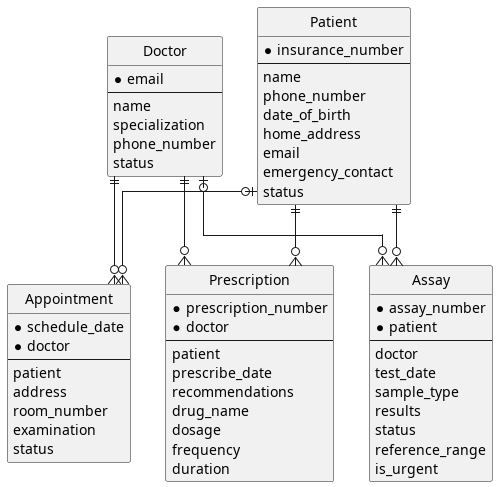
\includegraphics[width=0.9\textwidth]{Hospital ER Diagram}
\caption{ER-диаграмма системы «Поликлиника»}
\label{fig:er_diagram}
\end{figure}

\begin{figure}[h!]
\centering
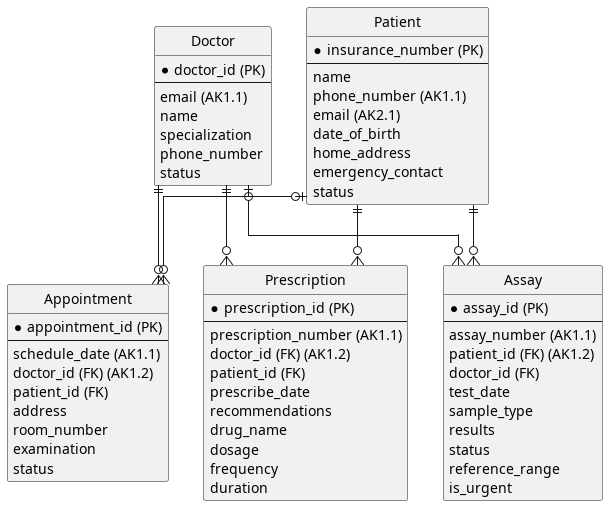
\includegraphics[width=0.9\textwidth]{Hospital Relational Diagram}
\caption{Реляционная модель системы «Поликлиника»}
\label{fig:rel_diagram}
\end{figure}

\clearpage

\paragraph{Таблицы отношений}

\begin{table}[h!]
\captionsetup{singlelinecheck=false, position=top}
\caption{Отношение Doctor (Врач)}
\begin{tabularx}{\textwidth}{|l|l|l|l|Y|}
\hline
  \textbf{Attribute Name} & \textbf{Type} & \textbf{Key} & \textbf{NULL Status} & \textbf{Remarks}\\
\hline
  doctor\_id & INT & PK & NOT NULL & Суррогатный ключ (PK)\\
\hline
email & VARCHAR(254) & AK(1.1) & NOT NULL & UNIQUE. Альтернативный ключ (AK1.1)\\
\hline
name & NVARCHAR(50) & AK(2.1) & NOT NULL & UNIQUE. Альтернативный ключ (AK2.1)\\
\hline
specialization & TINYINT & - & NOT NULL & Специализация врача: \newline
1 — терапевт \newline
2 — отоларинголог \newline
3 — невролог \newline
4 — офтальмолог \newline
5 — эндокринолог \newline
6 — хирург \newline
7 — дерматолог \newline
8 — психиатр \newline
9 — гастроэнтеролог \newline
10 — ревматолог \newline
\\
\hline
phone\_number & CHAR(11) & - & NULL & Контактный телефон (опционально)\\
\hline
status & TINYINT & - & NOT NULL & Статус: \newline
0 - не работает \newline
1 - работает \newline
2 - в отпуске \newline
3 - на больничном \newline
4 - в декрете
\\
\hline
\end{tabularx}
\end{table}

\begin{table}[h!]
\captionsetup{singlelinecheck=false, position=top}
\caption{Отношение Appointment (Приём)}
\begin{tabularx}{\textwidth}{|l|l|l|l|Y|}
\hline
	\textbf{Attribute Name} & \textbf{Type} & \textbf{Key} & \textbf{NULL Status} & \textbf{Remarks}\\
\hline
appointment\_id & INT & PK & NOT NULL & Суррогатный ключ (PK)\\
\hline
schedule\_date & DATETIME & AK(1.1) & NOT NULL & UNIQUE 1.1 Дата и время приёма (в составе AK1)\\
\hline
doctor\_id & INT & FK,AK(1.2) & NOT NULL & UNIQUE 1.2 Внешний ключ на Doctor (в составе AK1)\\
\hline
patient\_id & INT & FK & NULL & Внешний ключ на Patient (опционально)\\
\hline
address & NVARCHAR(75) & - & NULL & Адрес проведения приёма (например: 'Бригадирский пер., 14, Москва, к. 15')\\
\hline
room\_number & NVARCHAR(5) & - & NULL & Номер кабинета\\
\hline
examination & NVARCHAR(MAX) & - & NULL & Информация о осмотре\\
\hline
status & TINYINT & - & NOT NULL & Статус приёма: \newline
0 - не состоялся \newline
1 - состоялся \newline
2 - отменён
\\
\hline
\end{tabularx}
\end{table}

\begin{table}[h!]
\captionsetup{singlelinecheck=false, position=top}
\caption{Отношение Prescription (Рецепт)}
\begin{tabularx}{\textwidth}{|l|l|l|l|Y|}
\hline
  \textbf{Attribute Name} & \textbf{Type} & \textbf{Key} & \textbf{NULL Status} & \textbf{Remarks}\\
\hline
prescription\_id & INT & PK & NOT NULL & Суррогатный ключ (PK)\\
\hline
prescription\_number & INT & AK(1.1) & NOT NULL & UNIQUE. Номер рецепта (AK1.1)\\
\hline
doctor\_id & INT & FK & NOT NULL & Внешний ключ на Doctor\\
\hline
patient\_id & INT & FK & NOT NULL & Внешний ключ на Patient\\
\hline
prescribe\_date & DATE & - & NOT NULL & Дата выписки рецепта\\
\hline
recommendations & NVARCHAR(1000) & - & NULL & Рекомендации врача по приему препарата\\
\hline
drug\_name & NVARCHAR(50) & - & NOT NULL & Наименование препарата\\
\hline
dosage & NVARCHAR(25) & - & NOT NULL & Дозировка в собственных единицах\\
\hline
frequency & NVARCHAR(25) & - & NOT NULL & Частота приёма\\
\hline
duration & NVARCHAR(25) & - & NOT NULL & Длительность курса\\
\hline
\end{tabularx}
\end{table}

\begin{table}[h!]
\captionsetup{singlelinecheck=false, position=top}
\caption{Отношение Patient (Пациент)}
\begin{tabularx}{\textwidth}{|l|l|l|l|Y|}
\hline
  \textbf{Attribute Name} & \textbf{Type} & \textbf{Key} & \textbf{NULL Status} & \textbf{Remarks}\\
\hline
insurance\_number & CHAR(16) & PK & NOT NULL & Первичный ключ (PK)\\
\hline
name & NVARCHAR(50) & & NOT NULL & Имя/ФИО \\
\hline
phone\_number & CHAR(11) & AK(1.1) & NOT NULL & UNIQUE Контактный телефон (AK1.1)\\
\hline
email & VARCHAR(254) & AK(2.1) & NOT NULL & UNIQUE Почта (AK2.1)\\
\hline
date\_of\_birth & DATE & - & NULL & Дата рождения\\
\hline
home\_address & NVARCHAR(75) & - & NULL & Домашний адрес\\
\hline
emergency\_contact & CHAR(11) & - & NULL & Контакт для экстренной связи\\
\hline
status & TINYINT & - & NOT NULL & Статус пациента: \newline
0 - неактивен \newline
1 - активен \\
\hline
\end{tabularx}
\end{table}


\begin{table}[h!]
\captionsetup{singlelinecheck=false, position=top}
\caption{Отношение Assay (Анализ)}
\begin{tabularx}{\textwidth}{|l|l|l|l|Y|}
\hline
  \textbf{Attribute Name} & \textbf{Type} & \textbf{Key} & \textbf{NULL Status} & \textbf{Remarks}\\
\hline
assay\_id & INT & PK & NOT NULL & Суррогатный ключ (PK)\\
\hline
assay\_number & INT & AK(1.1) & NOT NULL & UNIQUE 1.1 Номер анализа (AK1.1)\\
\hline
patient\_id & INT & FK,AK(1.2) & NOT NULL & UNIQUE 1.2 Внешний ключ на Patient (в составе AK1)\\
\hline
doctor\_id & INT & FK & NULL & Внешний ключ на Doctor (опционально)\\
\hline
test\_date & DATE & - & NOT NULL & Дата взятия образца\\
\hline
sample\_type & TINYINT & - & NOT NULL & Тип образца: \newline 
1 - кровь \newline
2 - моча \newline
3 - слюна \newline
4 - кал \newline
5 - мокрота
\\
\hline
results & NVARCHAR(MAX) & - & NULL & Результаты анализа\\
\hline
status & TINYINT & - & NOT NULL & Статус анализа: \newline
0 - в процессе \newline
1 - завершен \newline
2 - отменен
\\
\hline
reference\_range & NVARCHAR(100) & - & NULL & Референсные значения в пределах нормы\\
\hline
is\_urgent & BIT & - & NOT NULL & Признак срочности\\
\hline
\end{tabularx}
\end{table}

\clearpage


\paragraph{Обоснование правил обеспечения ограничения минимальной кардинальности}

\begin{itemize}
  \item \textbf{Doctor к Appointment} - Идентифицирующая связь M-O, 1:N (см. таблицу \ref{table:DoctorAppointment})
  \item \textbf{Doctor к Prescription} - Идентифицирующая связь M-O, 1:N (см. таблицу \ref{table:DoctorPrescription})
  \item \textbf{Doctor к Assay} - Неидентифицирующая связь O-O, 1:N (см. таблицу \ref{table:DoctorAssay})
  \item \textbf{Patient к Appointment} - Неидентифицирующая связь O-O, 1:N (см. таблицу \ref{table:PatientAppointment})
  \item \textbf{Patient к Prescription} - Неидентифицирующая связь M-O, 1:N (см. таблицу \ref{table:PatientPrescription})
  \item \textbf{Patient к Assay} - Идентифицирующая связь M-O, 1:N (см. таблицу \ref{table:PatientAssay})
\end{itemize}


\begin{table}[h!]
\centering
\captionsetup{singlelinecheck=false, position=top}
\caption{Doctor к Appointment}
\begin{adjustbox}{max width=\textwidth}
\begin{tabular}{|p{0.22\textwidth}|p{0.36\textwidth}|p{0.36\textwidth}|}
\hline
\textbf{Операция} & \textbf{Действия над Doctor (родитель)} & \textbf{Действия над Appointment (ребёнок)} \\
\hline
Вставка & Без ограничений & Подбор родительской записи \\
\hline
Изменение & Запрещено -- суррогатный ключ & Разрешено -- принимающий врач может быть изменен \\
\hline
Удаление & Каскадное удаление приемов & Разрешено -- прием может быть отменен \\
\hline
\end{tabular}
\end{adjustbox}
\label{table:DoctorAppointment}
\end{table}

% --- Doctor to Prescription (identifying M-O, 1:N)
\begin{table}[h!]
\centering
\captionsetup{singlelinecheck=false, position=top}
\caption{Doctor к Prescription}
\begin{adjustbox}{max width=\textwidth}
\begin{tabular}{|p{0.22\textwidth}|p{0.36\textwidth}|p{0.36\textwidth}|}
\hline
	\textbf{Операция} & \textbf{Действия над Doctor (родитель)} & \textbf{Действия над Prescription (ребёнок)} \\
\hline
Вставка & Без ограничений & При создании рецепта задается врач \\
\hline
Изменение & Запрещено -- суррогатный ключ & Запрещено -- изменение врача выдавшего рецепт невозможно \\
\hline
Удаление & Запрещено -- рецепты должны остаться закреплены за врачом, который их выписал & Запрещено -- рецепты должны оставаться в истории \\
\hline
\end{tabular}
\end{adjustbox}
\label{table:DoctorPrescription}
\end{table}

% --- Doctor to Assay (non-identifying O-O, 1:N)
\begin{table}[h!]
\centering
\captionsetup{singlelinecheck=false, position=top}
\caption{Doctor к Assay}
\begin{adjustbox}{max width=\textwidth}
\begin{tabular}{|p{0.22\textwidth}|p{0.36\textwidth}|p{0.36\textwidth}|}
\hline
	\textbf{Операция} & \textbf{Действия над Doctor (родитель)} & \textbf{Действия над Assay (ребёнок)} \\
\hline
Вставка & Без ограничений & Пока врач не взял анализ, связь не устанавливается \\
\hline
Изменение & Запрещено -- суррогатный ключ & Разрешено -- привязка анализа к врачу может быть изменена или установлена позднее \\
\hline
Удаление & Запрещено -- нельзя удалить врача, так как анализ за ним закреплен & Запрещено -- все взятые анализы должны остаться в истории \\
\hline
\end{tabular}
\end{adjustbox} 
\label{table:DoctorAssay}
\end{table}

% --- Patient to Appointment (non-identifying O-O, 1:N)
\begin{table}[h!]
\centering
\captionsetup{singlelinecheck=false, position=top}
\caption{Patient к Appointment}
\begin{adjustbox}{max width=\textwidth}
\begin{tabular}{|p{0.22\textwidth}|p{0.36\textwidth}|p{0.36\textwidth}|}
\hline
	\textbf{Операция} & \textbf{Действия над Patient (родитель)} & \textbf{Действия над Appointment (ребёнок)} \\
\hline
Вставка & Без ограничений & Без ограничений \\
\hline
Изменение & Запрещено -- номер страховки & Разрешено -- пациент может быть изменен, так как пациенты записываются на места сами и могут отменять записи \\
\hline
Удаление & Разрешено -- запись пациента отменяется & Запрещено -- все записи привязаны к врачам и должны остаться, вне зависимости от пациентов \\
\hline
\end{tabular}
\end{adjustbox}
\label{table:PatientAppointment}
\end{table}

% --- Patient to Prescription (non-identifying M-O, 1:N)
\begin{table}[h!]
\centering
\captionsetup{singlelinecheck=false, position=top}
\caption{Patient к Prescription}
\begin{adjustbox}{max width=\textwidth}
\begin{tabular}{|p{0.22\textwidth}|p{0.36\textwidth}|p{0.36\textwidth}|}
\hline
	\textbf{Операция} & \textbf{Действия над Patient (родитель)} & \textbf{Действия над Prescription (ребёнок)} \\
\hline
Вставка & Без ограничений & Выбор родительской записи \\
\hline
Изменение & Запрещено -- номер страховки & Запрещено -- рецепт выдается конкретному пациенту \\
\hline
Удаление & Запрещено -- нельзя удалить пациента, рецепт закреплен за пациентом & Запрещено -- рецепты должны оставаться в истории \\
\hline
\end{tabular}
\end{adjustbox}
\label{table:PatientPrescription}
\end{table}

% --- Patient to Assay (identifying M-O, 1:N)
\begin{table}[h!]
\centering
\captionsetup{singlelinecheck=false, position=top}
\caption{Patient к Assay}
\begin{adjustbox}{max width=\textwidth}
\begin{tabular}{|p{0.22\textwidth}|p{0.36\textwidth}|p{0.36\textwidth}|}
\hline
	\textbf{Операция} & \textbf{Действия над Patient (родитель)} & \textbf{Действия над Assay (ребёнок)} \\
\hline
Вставка & Без ограничений & Подбор родительской записи \\
\hline
Изменение & Запрещено -- номер страховки & Запрещено -- анализ берется у конкретного пациента \\
\hline
Удаление & Запрещено -- анализы, закреплены за пациентом. & Запрещено -- анализы остаются в истории \\
\hline
\end{tabular}
\end{adjustbox}
\label{table:PatientAssay}
\end{table}
\end{document}